\chapter{\label{cha:background}Background \& Theory}

\section{Operator Learning}\label{sec:operator-learning}

Operator learning refers to the use of neural networks to approximate mappings between function spaces, rather than between finite-dimensional vectors as is done for classical neural network approaches \cite{neural-operators}. This setting arises naturally in scientific computing, where many problems can be formulated in terms of operators acting on functions.

A particularly important example is the solution operator of a parametric partial differential equation (PDE). Consider a PDE of the form:
\begin{equation}
\mathcal{N}(a, u)(x) = f(x), \quad x \in \Omega, \qquad u(x) = 0, \quad x \in \partial \Omega,
\end{equation}
where $\Omega \subset \mathbb{R}^d$ is a bounded domain, $\mathcal{N}$ is an operator, $a$ is an input function, $f$ is an external term like a forcing term, and $u$ is the solution.

The corresponding solution operator is defined as:
\begin{equation}
\mathcal{G}(a)(x) = u(x),
\end{equation}
which maps an input function $a$ to the solution $u$. The goal of operator learning is to approximate this mapping directly using surrogate modeling. 

Let $\mathcal{A}$ and $\mathcal{U}$ denote appropriate function spaces for the input and output, respectively. Given a dataset of input-output pairs:
\begin{equation}
\{(a_j, u_j)\}_{j=1}^{N_{\text{data}}}, \quad u_j = \mathcal{G}(a_j),
\end{equation}
where the inputs $a_j$ are sampled from a distribution $\mu$ over $\mathcal{A}$, the objective is to learn a parametric approximation $\mathcal{G}_\theta : \mathcal{A} \to \mathcal{U}$ by minimizing the expected error
\begin{equation}
\mathbb{E}_{a \sim \mu} \left[ \| \mathcal{G}(a) - \mathcal{G}_\theta(a) \|_{\mathcal{U}}^2 \right],
\end{equation}
which in practice is approximated by the empirical loss over the dataset.

A common theoretical formulation of neural operators represents each layer as
\begin{equation}
    \label{eq:og-formulation}
v_{\ell+1}(x)=\sigma\left(Wv_\ell(x)+\int_{\Omega}\kappa(x,y)v_\ell(y)\,dy\right),
\end{equation}
where $v_\ell(x)$ denotes the latent feature representation at spatial location $x$ in layer $\ell$, $W$ is a pointwise channel-mixing operator, $\kappa(x,y)$ is a learned kernel describing interactions between spatial locations $x$ and $y$, and $\sigma$ is a nonlinear activation function \cite{neural-operators}. Unlike standard neural network layers, which operate on fixed finite-dimensional vectors, this formulation acts on functions defined over a continuous domain through a global integral operator. In principle, this allows the learned mapping to depend on the underlying continuous function rather than on a specific discretization. In practice, however, neural operators are always trained on discretized samples of functions, and different architectures approximate this idealized formulation to different degrees.

A key distinction from standard learning problems is therefore that the objects of interest are continuous functions rather than finite-dimensional vectors, even though they are only observed through discrete samples. The learning problem is formulated at the level of a continuous operator, while training and inference are performed on discretized representations. Understanding what information about a function is preserved under discretization is therefore central to understanding discretization invariance in neural operators.

\subsection{Bandlimitedness and Continuous--Discrete Equivalence}\label{sec:bandlimitedness}

A central question in operator learning is what information about a continuous function is preserved when it is represented through discrete samples. Sampling theory provides a framework for answering this question, by characterizing when a function can be uniquely reconstructed from its values on a discrete grid.



Let $f \in L^2(\mathbb{R})$ be a square-integrable function with Fourier transform $\hat{f}$. The function is said to be bandlimited with bandlimit $\Omega > 0$ if its Fourier transform is supported only on a finite interval:
\begin{equation}
\mathrm{supp}(\hat{f}) \subset [-\Omega, \Omega].
\end{equation}

The Whittaker-Shannon sampling theorem states that a bandlimited function can be exactly reconstructed from its values on a uniform grid, provided the sampling rate is sufficiently high \cite{signals-and-systems}. Specifically, if the function is sampled at points $\{f(nT)\}_{n \in \mathbb{Z}}$, then exact reconstruction is possible if
\begin{equation}
\frac{1}{T} \geq 2\Omega,
\end{equation}
where $1/T$ is the sampling frequency and $2\Omega$ is called the Nyquist rate.

Under this condition, the function can be reconstructed via the interpolation formula
\begin{equation}
f(x) = \sum_{n \in \mathbb{Z}} f(nT)\,\mathrm{sinc}\left(\frac{x - nT}{T}\right),
\end{equation}
where $\mathrm{sinc}(x) = \frac{\sin(\pi x)}{\pi x}$.

This result establishes a form of continuous--discrete equivalence: if a function is bandlimited and sampled above the Nyquist rate, then its discrete samples contain all the information required to reconstruct the original function. In this case, the discretization is effectively lossless.

However, if the sampling rate is below the Nyquist rate, this equivalence breaks down. Different continuous functions can then produce the same values at the sampled points, so the original function can no longer be uniquely reconstructed from the discrete data. In Fourier terms, the unresolved high-frequency components do not remain separate from the resolved part of the spectrum. Instead, they appear on the sampled grid as lower-frequency components.

This misrepresentation of unresolved high-frequency content as lower-frequency content is known as aliasing. Intuitively, aliasing occurs when the function oscillates too rapidly relative to the spacing between sample points. The grid cannot represent this oscillation as a distinct high-frequency component, so it appears in the sampled data as a lower-frequency oscillation.

Figure~\ref{fig:aliasing} illustrates this effect. The blue curve represents a high-frequency signal, while the red curve is a lower-frequency function passing through the same sampled points. Since the sampled representation contains only the values at the black dots, both continuous functions correspond to the same discrete data. If the lower-frequency curve lies inside the range of frequencies that the grid can represent while the high-frequency curve lies outside it, the sampled representation interprets the high-frequency signal as its lower-frequency alias.

\begin{figure}
    \centering
    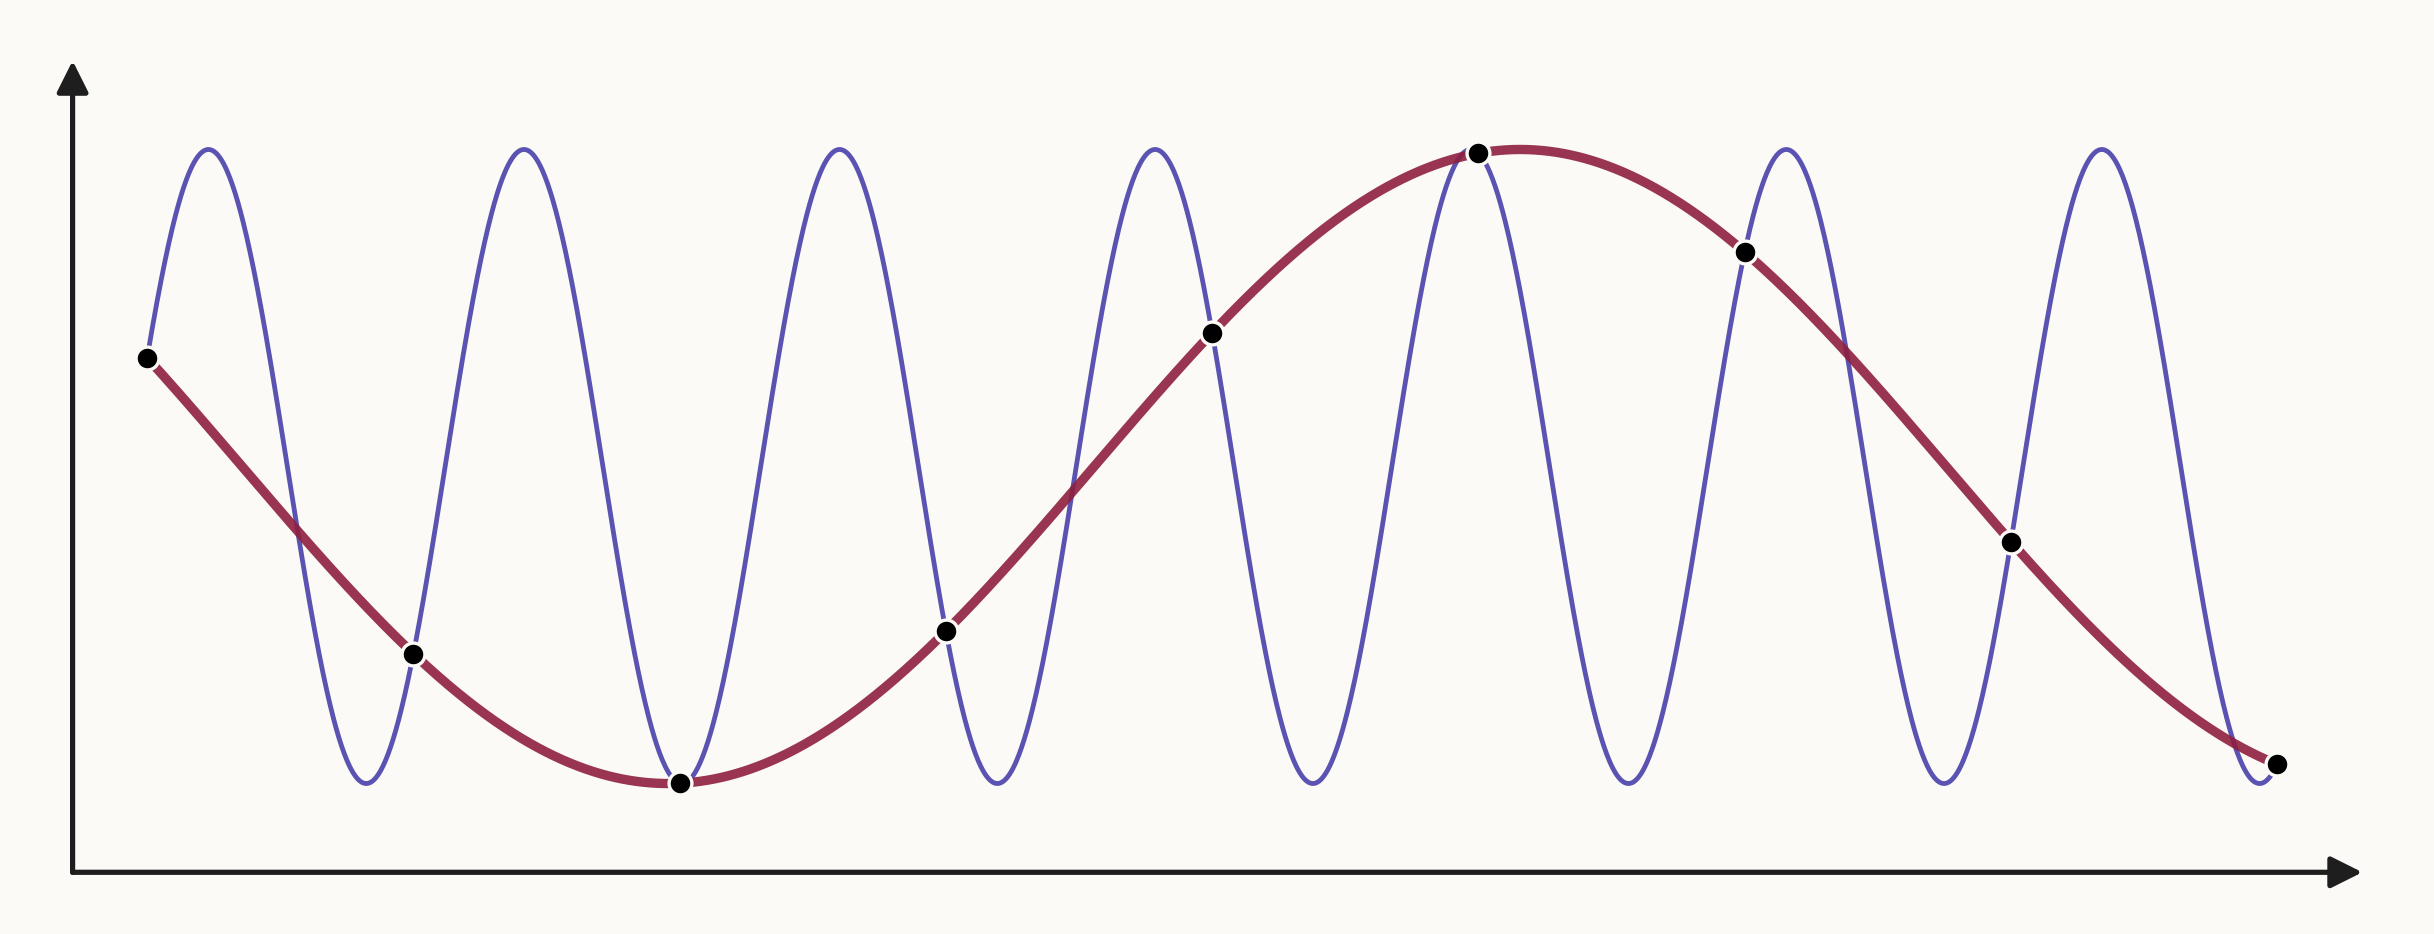
\includegraphics[width=0.8\textwidth]{figures/aliasing.png}
    \caption{\label{fig:aliasing} An illustration of aliasing. The blue curve represents a high-frequency signal, while the red curve is a lower-frequency function that passes through the same sampled points (black dots). Since both functions agree at the sampling locations, the discrete representation cannot distinguish between them.}
\end{figure}

From a Fourier perspective, once the sampling spacing \(T\) has been fixed, the grid has a maximum representable angular frequency. This is the Nyquist limit,
\begin{equation}
\omega_N = \frac{\pi}{T},
\end{equation}
where \(T\) is the spacing between sample points. Equivalently, \(\omega_N\) is half the sampling angular frequency \(2\pi/T\). Frequencies satisfying
\begin{equation}
|\omega| \leq \omega_N
\end{equation}
can be represented uniquely on the sampled grid, while frequencies above this limit cannot.

Consider a sinusoidal component
\begin{equation}
f(x) = \sin(\omega x).
\end{equation}
Sampling this function at points \(x_n = nT\) gives
\begin{equation}
f(nT) = \sin(\omega nT).
\end{equation}
The samples are unchanged when the frequency is shifted by an integer multiple of the sampling angular frequency \(2\pi/T\). Since \(2\omega_N = 2\pi/T\), frequencies of the form
\begin{equation}
\omega - 2k\omega_N, \qquad k \in \mathbb{Z},
\end{equation}
produce the same discrete oscillation after sampling. The represented frequency is obtained by choosing \(k\) so that the shifted frequency lies inside the Nyquist interval:
\begin{equation}
-\omega_N \leq \omega - 2k\omega_N \leq \omega_N.
\end{equation}
For a real-valued sinusoid, this is often reported as the non-negative aliased frequency
\begin{equation}
\omega_{\mathrm{alias}} = |\omega - 2k\omega_N|,
\end{equation}
with \(k\) chosen such that
\begin{equation}
0 \leq \omega_{\mathrm{alias}} \leq \omega_N.
\end{equation}

This mapping of frequencies outside the Nyquist interval back into the representable band is called folding. Sampling below the Nyquist rate therefore does not simply remove all frequency content above \(\omega_N\). Instead, unresolved high-frequency components are folded into lower represented frequencies. If several continuous Fourier components fold onto the same represented frequency, their complex Fourier coefficients contribute to the same discrete mode. Depending on their phases, these contributions may reinforce or partially cancel. The sampled data therefore contains a distorted spectrum in which unresolved high-frequency content contaminates modes that appear to be lower frequency.

The consequence is that information above the Nyquist limit is irreversibly lost as distinct high-frequency information. Once aliasing has occurred, the sampled data no longer contains enough information to determine whether a represented low-frequency mode came from a true low-frequency component, from unresolved high-frequency content, or from a combination of both. No learning algorithm can reconstruct frequency content that is absent from the discretized data, regardless of model complexity or architecture \cite{bartolucci-discretization-invariance}.

In the context of neural operators, aliasing can arise in two distinct ways. The first occurs during discretization of the original continuous function, when the sampling rate is insufficient to resolve the underlying frequency content. This form of aliasing is a property of the data representation itself and cannot be corrected after sampling has taken place. A second form of aliasing can occur inside the neural operator architecture. Nonlinear operations applied to bandlimited representations generate new higher-frequency components that may lie above the Nyquist limit of the internal discretization used by the model. If these components are not explicitly removed, they fold into the representable frequency range and alter the resolved modes. This architectural form of aliasing can therefore occur even when the original sampled input data is sufficiently resolved.


\subsection{Discretization Invariance}\label{sec:discretization-invariance}

The discussion in Section \ref{sec:bandlimitedness} shows that learning from discretized data is fundamentally constrained by the information preserved under sampling. Even if a model is intended to approximate a continuous operator, it is trained and evaluated on finite representations of functions. This raises the question of whether the learned model depends only on the underlying function, or also on the particular discretization used to represent it.

The desired property is referred to as discretization invariance. Informally, a discretization\hyp{}invariant model should produce consistent predictions when the same underlying function is represented on different grids, provided those discretizations sufficiently resolve the relevant features of the problem.

In practice, discretization invariance is most naturally interpreted for functions represented on uniform Cartesian grids, where resolution can be clearly defined through grid spacing. In this setting, it refers to the ability of a model trained at one resolution to make accurate predictions of the same underlying problem represented at other resolutions.

A widely used definition of neural operators is given by Kovachki et al. \cite{neural-operators}, stating that a neural operator should satisfy three key properties:

\begin{enumerate}
    \item \textbf{Discretization flexibility:} the model can accept inputs defined on arbitrary discretizations of the domain.
    
    \item \textbf{Pointwise evaluation:} the model can be evaluated at arbitrary output locations.
    
    \item \textbf{Continuum consistency:} as the discretization is refined, the learned operator converges to the underlying continuous operator being approximated.
\end{enumerate}

These properties formalize the idealized objective that a neural operator should approximate a mapping between functions. In this view, the learned operator should primarily depend on the underlying continuous object rather than on the particular resolution, ordering, or structure of the discretization used to represent it. In practice, however, many architectures still retain a significant dependence on the representation used during training.

This dependence becomes visible when the discretization is changed. If refining or otherwise changing the discretization changes the model output, the model is tied to the training representation rather than to the operator itself. As a result, performance may degrade significantly when evaluated on different resolutions or different discretizations of the same problem. This phenomenon is referred to as discretization mismatch \cite{gao-discretization-invariance}.

Discretization invariance is therefore a central criterion for evaluating neural operator architectures. In this thesis, it is used both as a theoretical concept and as an empirical measure for comparing models across changes in resolution.

\section{Fourier Neural Operator -- FNO}\label{sec:fno}

The Fourier Neural Operator (FNO), introduced by Li et al. \cite{li2021fno}, was the first major neural operator architecture to demonstrate strong performance on large-scale PDE learning problems and remains one of the most influential models in operator learning. Its success established neural operators as a practical alternative to classical numerical solvers and motivated much of the subsequent development in the field \cite{fno-explained}, including architectures such as the Convolutional Neural Operator (CNO) and geometry-aware Fourier Neural Operator (Geo-FNO).

\begin{figure}
    \centering
    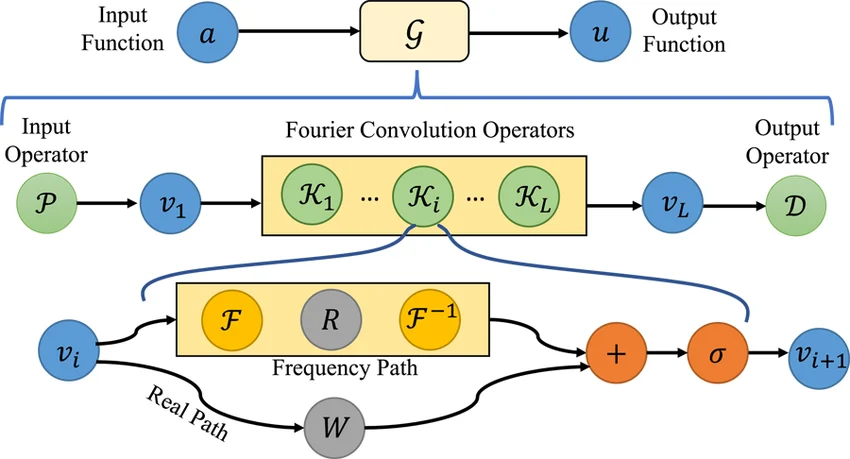
\includegraphics[width=0.8\textwidth]{figures/fno_figure.png}
    \caption{\label{fig:fno_architecture} The architecture of the Fourier Neural Operator (FNO), showing the lifting layer, repeated Fourier layers consisting of spectral convolution and pointwise channel mixing, and the final projection layer. \cite{fno-figure}.}
\end{figure}

The central idea of the FNO is to learn the solution operator in Fourier space. The model performs global convolution by transforming the input field into its Fourier representation, applying learned transformations to the Fourier coefficients, and transforming the result back to the spatial domain.

Figure~\ref{fig:fno_architecture} illustrates the architecture of the FNO. The model approximates the solution operator
\[
\mathcal{G}: a \mapsto u ,
\]
where $a$ is the input function and $u$ is the corresponding solution field. The full network consists of three main components: an input lifting operator, a sequence of Fourier layers, and an output projection operator.

The lifting operator maps the input field into a higher-dimensional latent representation,
\begin{equation}
\mathcal{P}: a(x) \rightarrow v_1(x),
\end{equation}
where $v_1(x)$ contains a larger number of feature channels than the original physical field. This allows the subsequent Fourier layers to operate in a richer latent space rather than directly on the low-dimensional physical variables.

The core of the architecture is the Fourier layer. Given an intermediate representation $v_l(x)$, each layer updates the features according to
\begin{equation}
v_{l+1}(x)
=
\sigma
\left(
Wv_l(x)
+
\mathcal{K}(v_l)(x)
\right),
\end{equation}
where $\mathcal{K}$ is the spectral convolution operator, $W$ is a pointwise linear transformation, and $\sigma$ is a nonlinear activation function.

The spectral convolution operator is implemented by first applying a Fourier transform to the input features that acts per channel, followed by truncation to a fixed number of low-frequency Fourier modes. For each retained mode, learned complex-valued weight matrices are applied to mix information across feature channels in frequency space. Finally, an inverse Fourier transform maps the result back to the spatial domain,
\begin{equation}
\mathcal{K}(v_l)
=
\mathcal{F}^{-1}
\left(
R \cdot \mathcal{F}(v_l)
\right),
\end{equation}
where $R$ denotes the learned complex weights acting on the retained modes as shown in Figure \ref{fig:fno_architecture}.

This frequency-space formulation is what distinguishes the FNO from standard convolutional architectures. Instead of learning kernels tied to a fixed spatial stencil, the model learns transformations of Fourier modes, which correspond to global basis functions spanning the entire domain.

Alongside the spectral path, the term $Wv_l(x)$ provides a local pointwise linear transformation in physical space. This is a channel-mixing operator analogous to a $1 \times 1$ convolution. It allows the model to incorporate local, pointwise corrections that cannot be represented by the truncated set of retained Fourier modes. Note that although $W$ and $\mathcal{K}$ are linear operations, the nonlinearity $\sigma$ allows the model to learn nonlinearities.

After several Fourier layers, the projection operator maps the final latent representation back to the physical output space,
\begin{equation}
\mathcal{D}: v_L(x) \rightarrow u(x),
\end{equation}
producing the predicted solution field.

\subsection{Strengths}

One of the main strengths of the FNO is its ability to capture global dependencies efficiently. Since Fourier modes are global basis functions, modifying a single coefficient influences the solution across the entire domain. This gives the model a global receptive field in every layer, making it particularly well suited for PDEs whose solution operators exhibit long-range interactions.

A second major advantage is computational efficiency. As discussed in Section~\ref{sec:operator-learning}, the theoretical neural operator formulation in Equation~\ref{eq:og-formulation} defines global interactions across the spatial domain through an integral operator. Directly evaluating the pairwise interactions implied by this formulation requires quadratic complexity in the number of spatial points $n$. The FNO avoids this cost by parameterizing the operator in Fourier space. By the convolution theorem, convolution in physical space is equivalent to pointwise multiplication in Fourier space. The spectral convolution can therefore be computed efficiently using the Fast Fourier Transform (FFT), reducing the computational complexity to
\begin{equation}
\mathcal{O}(n \log n),
\end{equation}
which makes large-scale operator learning computationally feasible.

The use of Fourier coefficients also provides a degree of resolution transfer across uniform Cartesian grids. Since the learned parameters act on modes rather than individual grid points, the same operator can be applied to different uniform resolutions without retraining, provided the relevant frequency content is sufficiently resolved. This makes the FNO significantly more flexible than standard convolutional networks, which are often strongly tied to the discretization used during training.

\subsection{Weaknesses}

The primary limitation of the FNO is its reliance on spectral truncation. In each Fourier layer, only a fixed number of low-frequency modes are retained, while the remaining higher\hyp{}frequency coefficients are discarded. This introduces an explicit architectural bandlimit determined by the number of retained modes.

This architectural bandlimit should be distinguished from the sampling bandlimit discussed in Section~\ref{sec:bandlimitedness}. In the sampling setting, frequencies above the Nyquist limit cannot be represented in the discretized data itself. In contrast, the FNO may discard higher\hyp{}frequency information even when those frequencies are present in the sampled input data, simply because they lie outside the retained set of Fourier modes. The architecture therefore imposes an additional spectral bottleneck beyond the limitations already introduced by discretization.

Another limitation concerns nonlinear aliasing. Pointwise nonlinear activations can generate frequency components that were not present in the input representation. If these components exceed the representable bandwidth of the discretized feature field, they cannot be resolved and instead appear as lower-frequency components through folding. This contaminates the resolved modes and can reduce the consistency of the learned representation across discretizations. 

A third important limitation is the reliance on uniform Cartesian grids. The standard FFT assumes regularly spaced points with consistent ordering, which makes the original FNO naturally suited for structured meshes but difficult to apply directly to irregular geometries or unstructured point clouds.




\section{Convolutional Neural Operator -- CNO} \label{sec:cno}

\subsection{Architecture}

\begin{figure}
    \centering
    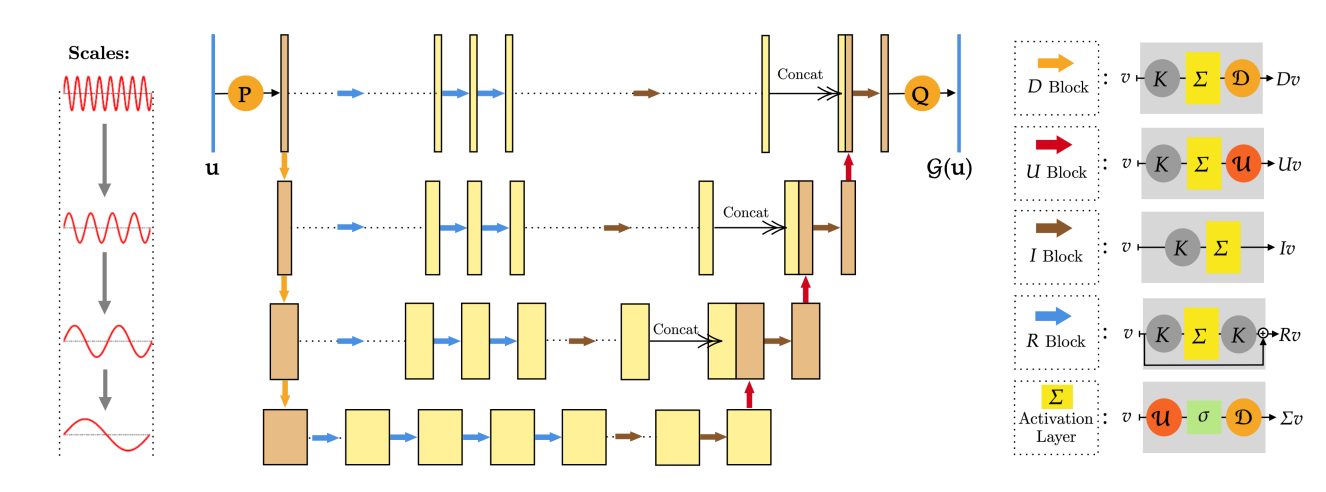
\includegraphics[width=0.8\textwidth]{figures/cno_figure.png}
    \caption{\label{fig:cno-architecture} The architecture of the Convolutional Neural Operator (CNO) \cite{cno}, showing the lifting operator $P$, projection operator $Q$, and the central U-shaped neural operator structure. The network combines downsampling ($D$-blocks), upsampling ($U$-blocks), residual blocks ($R$-blocks), and invariant blocks ($I$-blocks) across multiple spatial scales, with skip connections and concatenation used to preserve multiscale information. Anti-aliased downsampling and upsampling ensure resolution-invariant feature propagation across discretizations.}
\end{figure}

The Convolutional Neural Operator (CNO), introduced by Raonic et al. \cite{cno}, extends the classical U-Net architecture \cite{U-net} to the operator learning setting. U-Nets and related convolutional neural networks have been highly successful in fields such as image processing and segmentation due to their ability to efficiently capture local spatial structure through convolutional kernels \cite{U-net}. The CNO adopts this encoder--decoder structure while introducing several modifications aimed at satisfying the discretization invariance requirements discussed in Section~\ref{sec:discretization-invariance}.

Unlike the Fourier Neural Operator, which learns global interactions through Fourier modes, the CNO is built on standard convolutions in physical space. A convolutional kernel acts on a local neighborhood of points, producing a local operator rather than a global spectral one. This makes the model structurally similar to standard convolutional neural networks, but introduces an important challenge for operator learning: the physical meaning of a fixed kernel depends on the discretization.

For example, a $3 \times 3$ kernel applied on a coarse grid covers a much larger physical region than the same kernel on a fine grid. As a result, a standard CNN or U-Net is not naturally discretization invariant, since changing the resolution changes the effective operator being learned.

To address this, the CNO uses a multi-scale encoder--decoder architecture together with an initial resampling step onto a fixed internal resolution. Figure~\ref{fig:cno-architecture} illustrates the overall structure. After the initial resampling, the input is passed through a lifting layer, which maps the physical input field into a higher-dimensional feature space. This serves the same purpose as in the FNO, allowing the operator to be learned in a richer latent representation.

The lifted representation then enters the encoder, where it passes through a sequence of convolutional blocks. Each block consists of a convolution followed by a nonlinear activation. As the representation moves deeper into the encoder, the spatial resolution is progressively reduced through interpolation-based downsampling, while the number of feature channels is increased. Although the kernel size remains fixed, applying it at multiple resolutions allows the network to process information across different spatial scales.

At the coarsest level, the decoder progressively reconstructs the solution by upsampling the representation back to higher resolutions. After each upsampling step, another convolutional block is applied. Skip connections link encoder and decoder stages at matching resolutions, allowing fine-scale information from earlier layers to be reintroduced during reconstruction.

A key modification compared to a standard U-Net is the use of resampling onto a fixed internal grid before the main operator learning begins. Regardless of the input resolution, the model first interpolates the input onto the same internal discretization. This ensures that the convolutional kernels always act over the same physical scale inside the network.

This design also connects directly to the bandlimitedness discussion in Section~\ref{sec:bandlimitedness}. By choosing a fixed internal resolution, the CNO imposes an explicit bandlimit on the learned representation. Frequencies beyond this scale are removed during resampling, so the model always operates on a controlled frequency range.

A second major modification is the replacement of standard pointwise nonlinearities with the upsample--nonlinearity--downsample (UND) block. A standard pointwise activation applied directly on a finite grid is not representation-equivalent: even if the input is bandlimited, the nonlinearity generates new higher-frequency components that may lie above the Nyquist limit. These unresolved frequencies alias into lower modes, making the discrete nonlinear operator inconsistent with the corresponding continuous operator and violating the continuum consistency condition discussed in Section~\ref{sec:discretization-invariance}.

To address this, the CNO first upsamples the representation before applying the nonlinearity, creating spectral room for the newly generated frequencies to exist without immediately aliasing into the resolved modes. After the activation is applied, the representation is downsampled back to the original resolution using a low-pass filtering operation that removes the unresolved high-frequency content. Ideally, this filtering would be performed using the sinc interpolation filter implied by the Whittaker--Shannon sampling theorem, which provides exact reconstruction for bandlimited functions \cite{signals-and-systems}. In practice, this is approximated by a finite-support low-pass blur filter for computational efficiency, since exact sinc filtering is non-local and expensive to evaluate.

After the decoder stage, a projection layer maps the final latent representation back to the physical output space, producing the predicted solution field. Together, the fixed-grid resampling and the UND block are the central modifications that distinguish the CNO from a standard U-Net and make it suitable for operator learning across multiple discretizations.

\subsection{Strengths}

A major strength of the CNO is its strong local inductive bias. Since the model is built on standard convolutions in physical space, it naturally captures local interactions where the state at a point depends primarily on its immediate neighborhood. This is particularly well suited for many physical systems such as advection, diffusion, heat transfer, and turbulence-dominated flows, where local spatial structure plays a dominant role.

The encoder--decoder structure further allows the model to capture interactions across multiple physical scales. Coarse-resolution layers represent large-scale structures and long-range behavior, while fine-resolution layers preserve localized detail through skip connections. This is especially important for multiscale systems such as Navier--Stokes flow, where energy is transferred across a wide range of length scales and both global and local behavior must be represented simultaneously.

Another important advantage is robustness across resolutions. For the CNO, resampling onto a fixed internal grid is required for the convolutional kernels to retain the same physical meaning when the input resolution changes. Otherwise, a fixed-size kernel would correspond to different physical length scales on different grids. This consistency comes at the cost of an interpolation step, which is not lossless and may introduce artifacts or remove high-frequency information. The advantage of the CNO is therefore that it trades interpolation error for a fixed internal representation on which the learned convolutional operator can act consistently. When the internal resolution is sufficiently high for the relevant features of the problem, this trade-off can lead to substantially more stable behavior under resolution transfer.

The explicit treatment of bandlimiting also provides an important advantage compared to architectures where truncation occurs only implicitly. By controlling both resampling and nonlinear aliasing through the fixed internal grid and the UND block, the CNO avoids many of the spectral artifacts associated with unresolved high-frequency content. This improves continuum consistency and makes the model much closer to satisfying the definition of a true neural operator discussed in Section~\ref{sec:discretization-invariance} and in the work of Bertolucci et al. \cite{bartolucci-discretization-invariance}.

\subsection{Weaknesses}

A practical limitation of the CNO is its dependence on the chosen internal resolution. The resampling step improves consistency by enforcing a fixed internal representation, but this resolution must be selected when the model is built and remains fixed after training. This amounts to assuming that the chosen internal grid is sufficiently fine to represent the physically relevant features of the problem. If an input or target contains structures above the Nyquist limit of the internal grid, those structures cannot be represented faithfully after resampling: they are either removed by the low-pass filtering operation or, if insufficiently filtered, aliased into lower represented modes. In this case, the model may remain stable across resolutions, but it is stable with respect to an under-resolved internal representation.

This explicit truncation of high-frequency information is therefore both a strength and a weakness. While it improves robustness and discretization consistency, it can reduce accuracy for problems where sharp gradients, discontinuities, or fine-scale geometric details play a dominant role. In such cases, the CNO may sacrifice important local information in exchange for stability.

Another practical limitation is the reliance on interpolation during resampling. Both the initial resampling onto the fixed internal grid and the repeated upsampling and downsampling operations in the UND blocks introduce approximation errors. Ideally, these operations would be performed using exact sinc interpolation for bandlimited functions, but in practice finite-support approximations are used for computational efficiency, which can introduce errors.

Finally, while the CNO improves discretization invariance substantially compared to standard U-Nets, it is still not fully resolution-independent in practice. Its behavior remains tied to the chosen internal discretization, meaning that discretization robustness depends strongly on how well this internal representation matches the true frequency content of the underlying problem.


\section{Mesh-free Operator Learning and Geo-FNO}

\subsection{Motivation for Irregular Domains}

The neural operators introduced in Sections~\ref{sec:fno} and~\ref{sec:cno} assume that the input and output fields are represented on uniform Cartesian grids. While this assumption is convenient for both Fourier-based and convolutional architectures, it is often restrictive for scientific and engineering problems where the natural discretization of the domain is non-uniform.

A uniform grid can be an inefficient representation when the solution exhibits strong spatial variation only in localized regions. For example, a flow field containing sharp boundary layers or localized vortices may require very high resolution in a small part of the domain, while the remaining regions vary smoothly and can be represented accurately with far fewer points. Using a uniform Cartesian grid forces the entire domain to be sampled at the highest required resolution, leading to unnecessary computational cost and memory usage.

In many applications, the geometry itself also does not naturally conform to a rectangular grid. Examples include fluid flow around airfoils, structural mechanics on curved surfaces, porous media with irregular boundaries, and many reactor physics problems involving complex geometries \cite{irregular-data}. In such settings, the natural discretization is often given by an unstructured mesh or a point cloud rather than a regular lattice.

A common workaround is to interpolate the data from the original mesh onto a uniform Cartesian grid and then apply a standard neural operator such as the FNO or CNO \cite{li2021fno}. However, this interpolation step introduces additional approximation error and may discard important geometric information contained in the original discretization. In particular, regions requiring high local resolution may be smoothed or under-resolved when forced onto a regular grid, reducing both accuracy and efficiency.

These limitations motivate the development of mesh-free neural operators, which aim to learn directly from irregular point clouds or unstructured meshes without requiring interpolation onto a Cartesian grid. Such models seek to preserve the geometric information present in the original discretization while retaining the advantages of operator learning.

\subsection{Geometry-aware Fourier Neural Operator -- geo-FNO}

\subsubsection{Architecture}

The geometry-aware Fourier Neural Operator (Geo-FNO), introduced by Li et al. \cite{geo-fno}, extends the original FNO to problems defined on irregular domains such as point clouds and unstructured meshes. While the standard FNO assumes that the input field is represented on a uniform Cartesian grid, Geo-FNO is designed to work directly with non-uniformly sampled input data.

Conceptually, Geo-FNO can be viewed as a generalization of the original FNO. The core Fourier Neural Operator remains unchanged: the model performs spectral convolution by transforming the input into Fourier space, applying learned complex weights to the retained modes, and transforming back to the spatial domain. The main modification is the introduction of a learned coordinate transformation placed before the FNO, together with non-uniform Fourier transforms at the input and output stages.

It is useful to distinguish between three different coordinate systems used in the model. The first is the input grid, corresponding to the original irregular point cloud where the data is given. The second is the computational grid, obtained after applying the learned coordinate transformation $\phi^{-1}$. This grid is still non-uniform, but is mapped into a representation that is more suitable for Fourier learning. The notation $\phi^{-1}$ is used to reflect that the learned transformation maps from the physical (irregular) domain to a more structured computational representation. In classical settings, a mapping $\phi$ is typically defined from a reference or structured domain to a physical domain, and the operation required here is therefore its inverse. In practice, only $\phi^{-1}$ is learned and used; the forward map $\phi$ is never explicitly constructed. The third coordinate system is the internal grid, which is the uniform Cartesian grid used within the FNO after the first spectral layer.

The learned coordinate transformation is denoted by $\phi^{-1}$, implemented in the original work as the network \texttt{IPHI}, short for inverse \(\phi\). Given input coordinates \(x\), and optionally a vector of geometry parameters \(g\), the mapping is defined as
\begin{equation}
\phi^{-1}(x, g) = x + f(x, g),
\end{equation}
where \(g\) denotes finite-dimensional information describing the geometry of the sample rather than an additional spatial coordinate. Such parameters can describe global features of the domain, for example the position, size, or shape of obstacles or boundaries. Their purpose is to condition the coordinate transformation on the specific geometry of each sample, allowing the same transformation network to adapt its mapping across different domains. A standard example from aerodynamic shape optimization is airfoil parameterization, where a continuous airfoil boundary is represented by a finite vector of shape coefficients; changing the entries of this vector changes the global airfoil geometry while the spatial coordinates \(x\) still denote points in the physical domain~\cite{airfoils}. \(f(x,g)\) is represented by a lightweight multilayer perceptron\footnote{The MLP is described as lightweight because, in the implementation used here, it consists of only three layers with width 32 and acts only on point coordinates and optional geometry parameters.} and initialized close to zero so that the mapping begins near the identity transformation. The coordinate transform is trained jointly with the FNO and learns a mapping that minimizes the prediction error while adapting to the geometry of the problem.

Importantly, this is a continuous-to-continuous mapping rather than interpolation onto a discrete grid. The transformed points remain irregularly distributed, and the purpose of the mapping is not to force the domain onto a regular mesh, but to provide a coordinate system in which Fourier-based operator learning becomes more effective.

After this transformation, the input field is processed using a non-uniform discrete Fourier transform rather than the standard FFT used in the original FNO. The resulting Fourier representation is then reconstructed on a uniform internal grid. After this step, the remaining Fourier layers operate as in the standard FNO using FFT-based spectral convolutions. Thus, the expensive non-uniform transforms are used only at the interface between the irregular point cloud and the uniform internal representation, while the main operator learning takes place on the regular internal grid.

At the output stage, the model can be evaluated at arbitrary physical query locations. These query points are passed through the same learned transformation \(\phi^{-1}\), mapping them into the computational coordinate system. The final spectral representation is then evaluated at the transformed query coordinates, producing the predicted solution values at the corresponding physical points. Since both input and output coordinates are mapped from the physical domain into the computational coordinate system, the model does not require an explicit forward map \(\phi\).

This means that Geo-FNO satisfies two of the three neural operator conditions discussed in Section~\ref{sec:discretization-invariance}: it can accept inputs defined on irregular point sets and can be evaluated at arbitrary output positions.



\subsubsection{Strengths}

The primary strength of Geo-FNO is that it extends Fourier-based operator learning to irregular domains without requiring the full problem to be pre-interpolated onto a Cartesian grid before learning begins. This allows the model to work directly on point clouds and unstructured meshes while preserving geometric information that may be lost during interpolation to a regular lattice.

Because the internal operator remains an FNO, Geo-FNO retains many of the advantages of spectral operator learning. It still benefits from global receptive fields, efficient FFT-based convolutions in the internal layers, and strong performance on operators dominated by large-scale smooth structure. Compared to fully mesh-based or graph-based approaches, this often provides significantly better computational efficiency.

The learned coordinate transform provides an important representational advantage. Rather than relying on a fixed hand\hyp{}designed mapping, the model learns a problem\hyp{}dependent coordinate system jointly with the operator itself. This allows the geometry to be adapted so that the retained low Fourier modes capture more of the physically relevant information, improving approximation quality without requiring a large increase in retained modes.

Another important strength is output flexibility. Since predictions are reconstructed from Fourier coefficients rather than tied to a fixed output mesh, the model can be evaluated at arbitrary query locations. This is particularly useful for scientific computing problems where predictions may be required on boundary points, locally refined meshes, or point-cloud discretizations not seen during training.


\subsubsection{Weaknesses}

The main limitation of the Geo-FNO is that it inherits many of the weaknesses of the original FNO. Spectral truncation remains central to the architecture, meaning that high-frequency information is still discarded and the model retains a strong low-frequency bias. For problems dominated by sharp gradients, discontinuities, or highly localized effects, this can still lead to poor approximation quality.

A second challenge arises from the use of non-uniform Fourier transforms. On a uniform Cartesian grid, the discrete Fourier basis vectors are orthogonal with respect to the discrete inner product over the grid points. As a result, each Fourier coefficient can be interpreted as the amplitude of a specific frequency mode, and truncating high modes has a clear meaning: selected frequencies are removed from the representation.

On an irregular point cloud, this discrete orthogonality no longer holds in general \cite{nonuniform-fft}. The Fourier basis functions evaluated at the sampled points are not mutually orthogonal under the corresponding discrete sum, so the coefficient associated with one nominal mode can contain contributions from other modes. As a result, truncating a coefficient no longer corresponds as cleanly to removing one specific frequency component, and applying a learned weight to that coefficient affects a less directly interpretable mixture of spectral information. This reduces the spectral interpretability of the non-uniform transform compared with the standard FFT on a uniform grid.

A further limitation is that the success of Geo-FNO depends heavily on the learned coordinate transform. If the mapping learned by $\phi^{-1}$ fails to produce a representation where the retained low Fourier modes are sufficiently informative, the model may still suffer from poor truncation behavior. Since this mapping is learned jointly with the FNO, training can become sensitive to initialization and optimization choices.

Although Geo-FNO avoids explicit pre-interpolation onto a Cartesian grid, it does not completely remove representation dependence. The quality of the learned operator still depends strongly on the spatial distribution of the input points. Poor geometric coverage, highly clustered sampling, or insufficient resolution near important local features may all produce unstable spectral representations, even after coordinate transformation. As a result, model performance depends not only on how many points are available, but critically on where those points are located relative to the underlying physics.

\section{Discretization Invariance on Mesh-Free Grids} \label{mesh-free-discretization-invariance}

So far, discretization invariance has primarily been discussed in the context of functions represented on uniform Cartesian grids. In that setting, the concept is relatively straightforward: increasing the resolution corresponds to decreasing the grid spacing uniformly while preserving the same underlying domain. A model can therefore be tested by training on one resolution and evaluating on another, allowing discretization invariance to be interpreted as robustness to resolution transfer.

For non-uniform meshes and point clouds, the notion of resolution is more involved. Such discretizations can still be assigned measures of resolution, for example through the number of points, maximum element diameter, average point spacing, or local sampling density. However, these quantities do not define a single canonical refinement parameter in the same way as the grid size \(N\) does on a uniform Cartesian grid. The quality of the discretization depends not only on how many points are used, but also on where they are placed relative to boundaries, geometric features, and regions where the solution varies rapidly. A point cloud with dense sampling near sharp gradients or boundaries may resolve the solution better than another point cloud with more points but poor placement.

In the mesh-free setting, discretization robustness is therefore better understood as robustness to changes in sampling geometry. The underlying PDE and continuous solution operator remain the same, but the model observes that problem through different point distributions or mesh refinements. The relevant question is whether the model produces consistent and accurate predictions when the same continuous problem is represented by different irregular discretizations.

A direct analogue of the uniform-grid resolution-transfer experiments would require controlled families of meshes or point clouds for the same underlying physical samples. For example, an unstructured triangular mesh can be systematically refined by subdividing its elements, while point clouds can be generated with prescribed changes in local sampling density. The mesh-free datasets used in this thesis were not generated with such controlled refinement families. With the available data, the only direct modification would be to subsample or otherwise change the number of points from the existing point clouds. This would not provide a controlled measure of discretization invariance, because changes in point count would be entangled with changes in point placement, local resolution, and interpolation or subsampling artifacts.

For this reason, the Geo-FNO evaluation focuses instead on whether the model can produce physically meaningful predictions directly on irregular point clouds and non-uniform meshes. Successful prediction in this setting does not by itself demonstrate full discretization invariance in the mesh-free sense, but it does test whether the model can learn on the original irregular representation without first interpolating the data onto a uniform Cartesian grid.




